\documentclass[10pt, aspectratio=169]{beamer}
\usepackage{tikz}
\usepackage{xurl}
\usetikzlibrary{shapes, arrows.meta, positioning}
% [aspectratio=169]
% 中文
\usepackage{xeCJK}
\setCJKmainfont{Noto Sans CJK TC}

\usetheme{metropolis}
\usepackage{appendixnumberbeamer}

\usepackage{booktabs}
\usepackage[scale=2]{ccicons}

\usepackage{pgfplots}
\usepgfplotslibrary{dateplot}

\usepackage{xspace}
\newcommand{\themename}{\textbf{\textsc{metropolis}}\xspace}

\title{Amazon智慧倉庫}
\subtitle{物聯網與手機無線控制期中報告}
% \date{\today}
\date{}
\author{S11182049 陳忠何}

\institute{}
% \titlegraphic{\hfill
\includegraphics[height=1.5cm]{logo.pdf}}

\begin{document}

\maketitle

\begin{frame}{Table of contents}
  \setbeamertemplate{section in toc}[sections numbered]
  \tableofcontents[hideallsubsections]
\end{frame}

\section{簡介}

\begin{frame}[fragile]{系統概念}
  \begin{columns}
    \column{0.5\textwidth}
      Amazon倉儲中心透過先進的機器人與AI技術,實現了自動化、高效率的物流管理。
    \column{0.5\textwidth}
      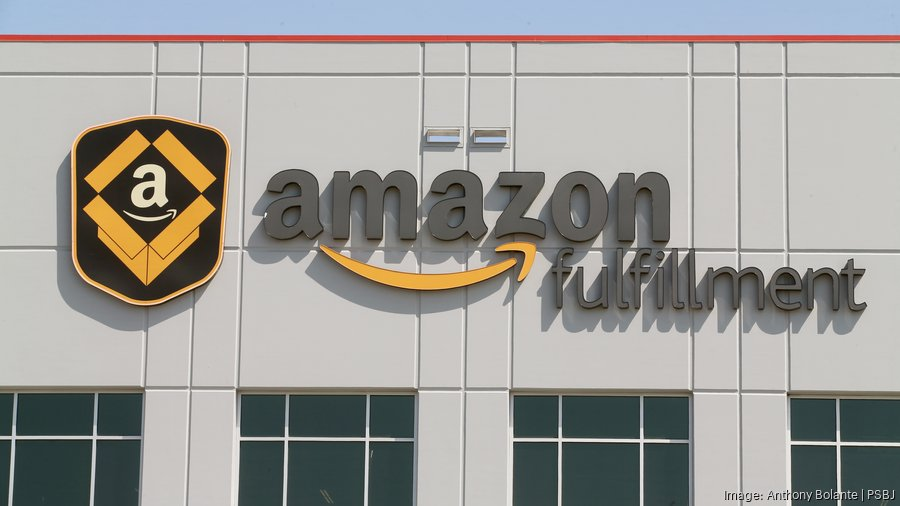
\includegraphics[width=\textwidth]{images/amazon-fulfillment-center.jpg}
  \end{columns}
\end{frame}
% 
\begin{frame}{Amazon 倉儲系統流程圖}
    \centering
    \begin{tikzpicture}[node distance=1.2cm, auto]
        % 定義每個流程方塊的樣式
        \tikzstyle{process} = [rectangle, rounded corners, minimum width=2.5cm, minimum height=0.8cm, text centered, draw=black, fill=blue!20]
        \tikzstyle{decision} = [diamond, minimum width=2cm, minimum height=0.8cm, text centered, draw=black, fill=orange!20]
        \tikzstyle{arrow} = [thick, ->, >=stealth]

        % Step 1: 供應商送貨
        \node (supplier) [process] {商品送到倉庫};

        % Step 2: Amazon Aurora 管理庫存
        \node (aurora) [process, right=of supplier, xshift=-0.5cm] {機器人移動貨架};

        % Step 3: 機器人儲存與掃描
        \node (robot_storage) [process, right=of aurora, xshift=-0.5cm] {工作人員掃描商品紀錄數量};


        % 繪製箭頭
        \draw [arrow] (supplier) -- (aurora);
        \draw [arrow] (aurora) -- (robot_storage);

    \end{tikzpicture}
\end{frame}
\begin{frame}{Amazon 倉儲系統流程圖}
    \centering
    \begin{tikzpicture}[node distance=1.2cm, auto]
        % 定義每個流程方塊的樣式
        \tikzstyle{process} = [rectangle, rounded corners, minimum width=2.5cm, minimum height=0.8cm, text centered, draw=black, fill=blue!20]
        \tikzstyle{decision} = [diamond, minimum width=2cm, minimum height=0.8cm, text centered, draw=black, fill=orange!20]
        \tikzstyle{arrow} = [thick, ->, >=stealth]

        % Step 1: 供應商送貨
        \node (order) [process] {用戶下訂單};

        % Step 2: Amazon Aurora 管理庫存
        \node (aurora) [process, right=of order, xshift=-0.5cm] {機器人移動貨架};

        % Step 3: 機器人儲存與掃描
        \node (robot_storage) [process, right=of aurora, xshift=-0.5cm] {工作人員將商品取出};

        % Step 4: Amazon Neptune 管理庫存
        \node (neptune) [process, right=of robot_storage, xshift=-0.5cm] {送到包裝線};

        % step 5: 貨物裝箱
        \node (pack) [process, below=of neptune, xshift=-0.5cm] {貨物裝箱};
        \node (ship) [process, left=of pack, xshift=-0.5cm] {貨物運送};

        % 繪製箭頭
        \draw [arrow] (supplier) -- (aurora);
        \draw [arrow] (aurora) -- (robot_storage);
        \draw [arrow] (robot_storage) -- (neptune);
        \draw [arrow] (neptune) -- (pack);
        \draw [arrow] (pack) -- (ship);
    \end{tikzpicture} 

\end{frame}


\begin{frame}[fragile]{設計動機與目標}
  \begin{itemize}
    \item 提高倉庫管理效率
    \item 降低人力成本
    \item 提高客戶滿意度
  \end{itemize}
\end{frame}

\begin{frame}[fragile]{客群}
  \begin{itemize}
    \item 全球範圍內的線上購物者
    \item Amazon賣家
    \item 供應商
  \end{itemize}
\end{frame}

\section{功能構成元素}

\begin{frame}{高效庫存管理}
  \begin{itemize}
    \item Amazon Aurora關聯式資料庫管理系統\\
      兼容MySQL和PostgreSQL,且效能更好。
    \item Amazon Neptune圖形資料庫管理系統\\
      可以儲存數十億個商品關係,並以毫秒級的延遲查詢圖形。
  \end{itemize}
\end{frame}

{
    \metroset{titleformat frame=smallcaps}
\begin{frame}{機器人}
  \begin{columns}
    \column{0.5\textwidth}
      Amazon Robotics負責貨物的搬運、定位、及工作站的供貨流程。
    \column{0.5\textwidth}
      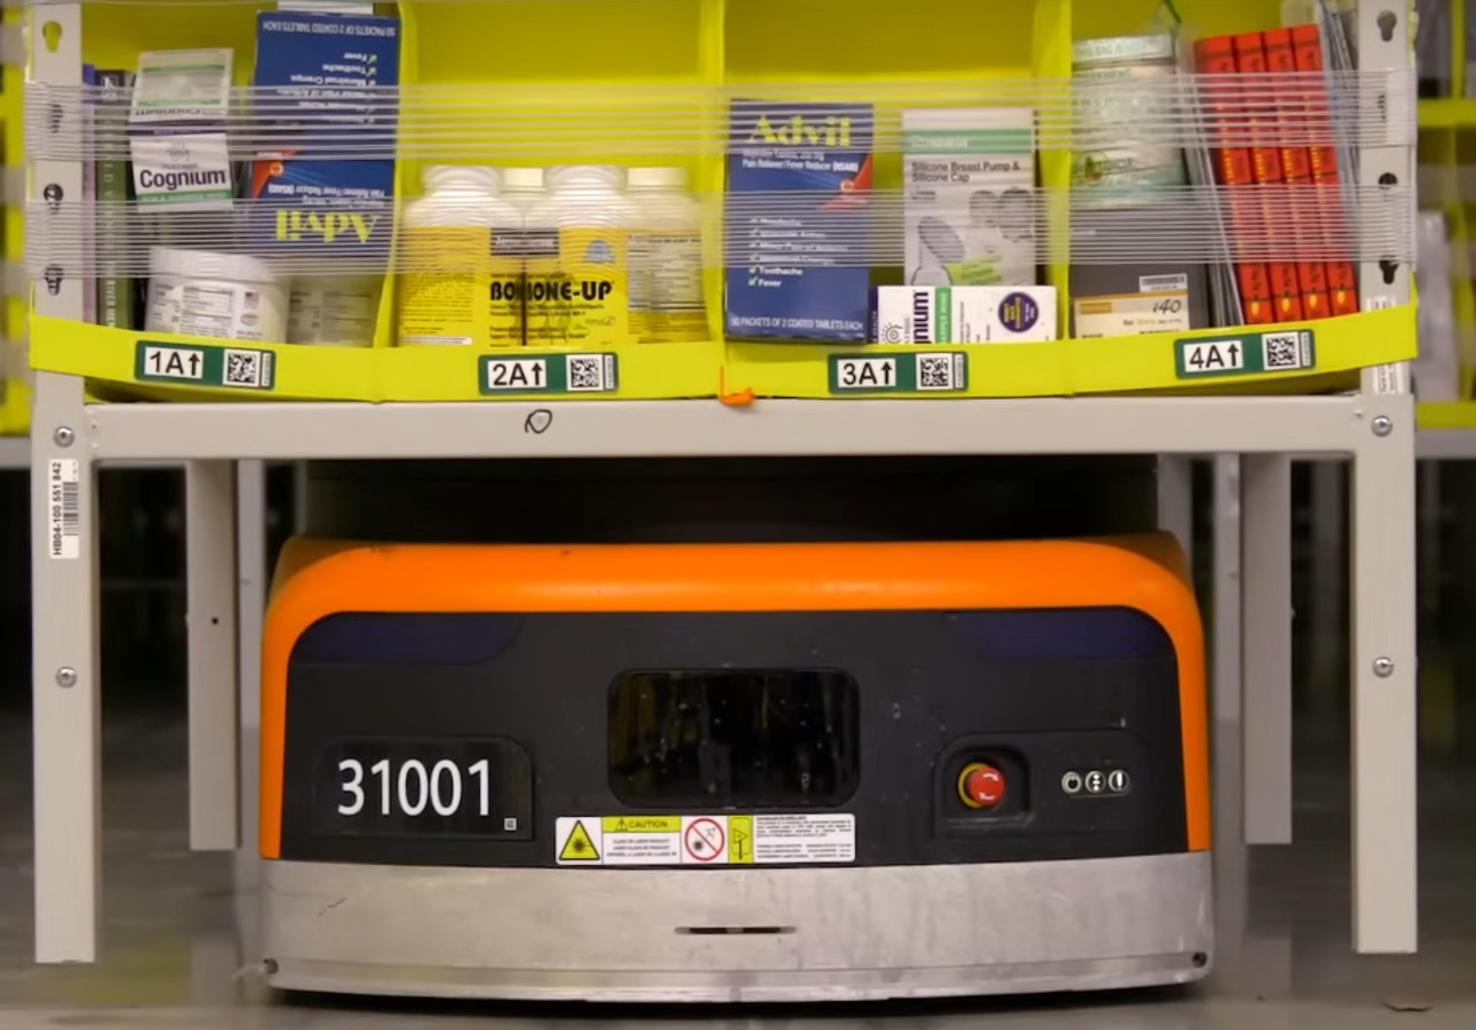
\includegraphics[width=\textwidth]{images/amazon-robotics.png}
  \end{columns}
	
\end{frame}
}
\begin{frame}{安全防護}
  \centering
  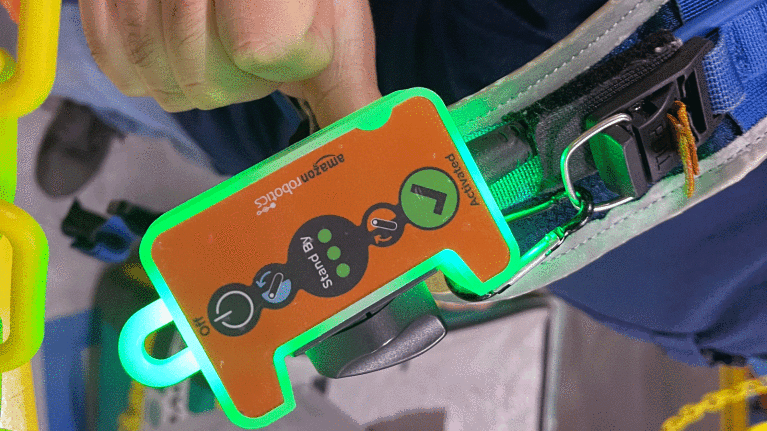
\includegraphics[width=0.8\textwidth]{images/amazon-vest.png}
\end{frame}

{
\metroset{titleformat frame=allsmallcaps}
\begin{frame}{電腦視覺系統}
  \begin{columns}
    \column{0.5\textwidth}
      應用於貨艙物品監測、提醒和物品數量確認。
    \column{0.5\textwidth}
      \centering
      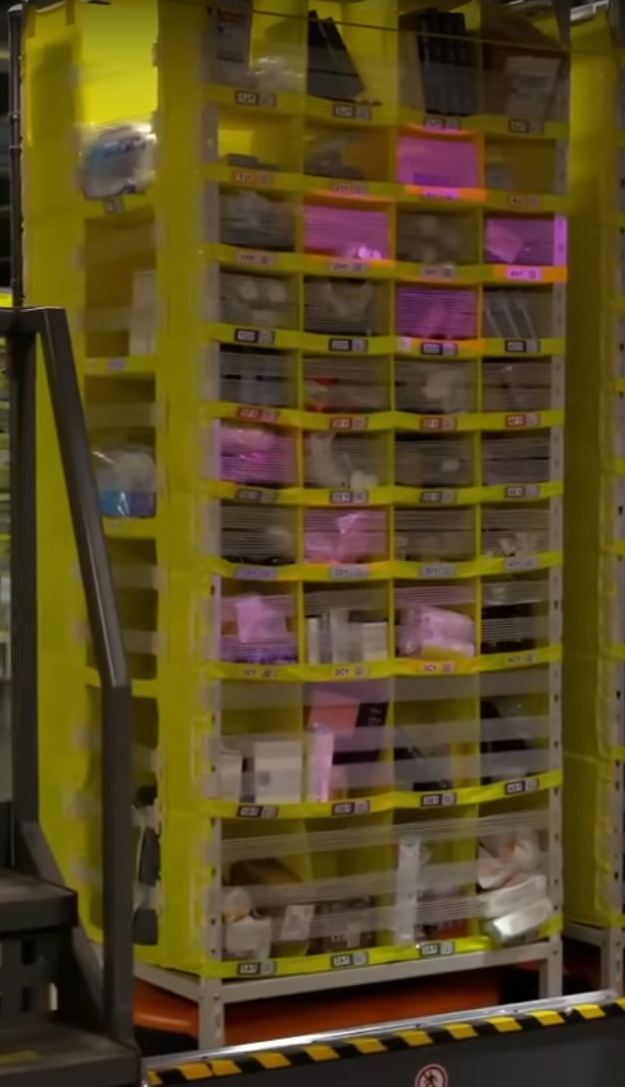
\includegraphics[width=0.5\textwidth]{images/amazon-pod-lights.png}
  \end{columns}
	
\end{frame}
}

{
\metroset{titleformat frame=allcaps}
\begin{frame}{SLAM}
  \begin{columns}
    \column{0.5\textwidth}
  \begin{itemize}
    \item Scan
    \item Label
    \item Apply
    \item Manifest
  \end{itemize}
    \column{0.5\textwidth}
      \centering
      \includegraphics[width=0.5\textwidth]{images/amazon-SLAM.jpg}
\end{columns}
\end{frame}
}

\section{成功因素及痛點}

\begin{frame}[fragile]{成功因素}
  \begin{itemize}
    \item 高效自動化技術
    \item 精確的物流管理
    \item 物流快速
  \end{itemize}
\end{frame}
\begin{frame}{現有痛點}
  \begin{itemize}
    \item 成本高昂
    \item 還是需要大量人力
  \end{itemize}  
\end{frame}

% \begin{frame}{Font feature test}
%   \begin{itemize}
%     \item Regular
%     \item \textit{Italic}
%     \item \textsc{Small Caps}
%     \item \textbf{Bold}
%     \item \textbf{\textit{Bold Italic}}
%     \item \textbf{\textsc{Bold Small Caps}}
%     \item \texttt{Monospace}
%     \item \texttt{\textit{Monospace Italic}}
%     \item \texttt{\textbf{Monospace Bold}}
%     \item \texttt{\textbf{\textit{Monospace Bold Italic}}}
%   \end{itemize}
% \end{frame}


% \begin{frame}{Figures}
%   \begin{figure}
%     \newcounter{density}
%     \setcounter{density}{20}
%     \begin{tikzpicture}
%       \def\couleur{alerted text.fg}
%       \path[coordinate] (0,0)  coordinate(A)
%                   ++( 90:5cm) coordinate(B)
%                   ++(0:5cm) coordinate(C)
%                   ++(-90:5cm) coordinate(D);
%       \draw[fill=\couleur!\thedensity] (A) -- (B) -- (C) --(D) -- cycle;
%       \foreach \x in {1,...,40}{%
%           \pgfmathsetcounter{density}{\thedensity+20}
%           \setcounter{density}{\thedensity}
%           \path[coordinate] coordinate(X) at (A){};
%           \path[coordinate] (A) -- (B) coordinate[pos=.10](A)
%                               -- (C) coordinate[pos=.10](B)
%                               -- (D) coordinate[pos=.10](C)
%                               -- (X) coordinate[pos=.10](D);
%           \draw[fill=\couleur!\thedensity] (A)--(B)--(C)-- (D) -- cycle;
%       }
%     \end{tikzpicture}
%     \caption{Rotated square from
%     \href{http://www.texample.net/tikz/examples/rotated-polygons/}{texample.net}.}
%   \end{figure}
% \end{frame}
% \begin{frame}{Tables}
%   \begin{table}
%     \caption{Largest cities in the world (source: Wikipedia)}
%     \begin{tabular}{@{} lr @{}}
%       \toprule
%       City & Population\\
%       \midrule
%       Mexico City & 20,116,842\\
%       Shanghai & 19,210,000\\
%       Peking & 15,796,450\\
%       Istanbul & 14,160,467\\
%       \bottomrule
%     \end{tabular}
%   \end{table}
% \end{frame}
% \begin{frame}{Blocks}
%   Three different block environments are pre-defined and may be styled with an
%   optional background color.

%   \begin{columns}[T,onlytextwidth]
%     \column{0.5\textwidth}
%       \begin{block}{Default}
%         Block content.
%       \end{block}

%       \begin{alertblock}{Alert}
%         Block content.
%       \end{alertblock}

%       \begin{exampleblock}{Example}
%         Block content.
%       \end{exampleblock}

%     \column{0.5\textwidth}

%       \metroset{block=fill}

%       \begin{block}{Default}
%         Block content.
%       \end{block}

%       \begin{alertblock}{Alert}
%         Block content.
%       \end{alertblock}

%       \begin{exampleblock}{Example}
%         Block content.
%       \end{exampleblock}

%   \end{columns}
% \end{frame}


% \begin{frame}{Line plots}
%   \begin{figure}
%     \begin{tikzpicture}
%       \begin{axis}[
%         mlineplot,
%         width=0.9\textwidth,
%         height=6cm,
%       ]

%         \addplot {sin(deg(x))};
%         \addplot+[samples=100] {sin(deg(2*x))};

%       \end{axis}
%     \end{tikzpicture}
%   \end{figure}
% \end{frame}
% \begin{frame}{Bar charts}
%   \begin{figure}
%     \begin{tikzpicture}
%       \begin{axis}[
%         mbarplot,
%         xlabel={Foo},
%         ylabel={Bar},
%         width=0.9\textwidth,
%         height=6cm,
%       ]

%       \addplot plot coordinates {(1, 20) (2, 25) (3, 22.4) (4, 12.4)};
%       \addplot plot coordinates {(1, 18) (2, 24) (3, 23.5) (4, 13.2)};
%       \addplot plot coordinates {(1, 10) (2, 19) (3, 25) (4, 15.2)};

%       \legend{lorem, ipsum, dolor}

%       \end{axis}
%     \end{tikzpicture}
%   \end{figure}
% \end{frame}


% \begin{frame}{References}
%   Some references to showcase [allowframebreaks] \cite{knuth92,ConcreteMath,Simpson,Er01,greenwade93}
% \end{frame}

\section{天馬行空的想像}
\begin{frame}{天馬行空的想像\&進化}
  \begin{columns}
  \column{0.4\textwidth}  
    \begin{itemize}
      \item 利用無人機在倉庫內部運送貨物
      \item 自動裝箱機器人
    \end{itemize}
  \column{0.6\textwidth}
    \centering
    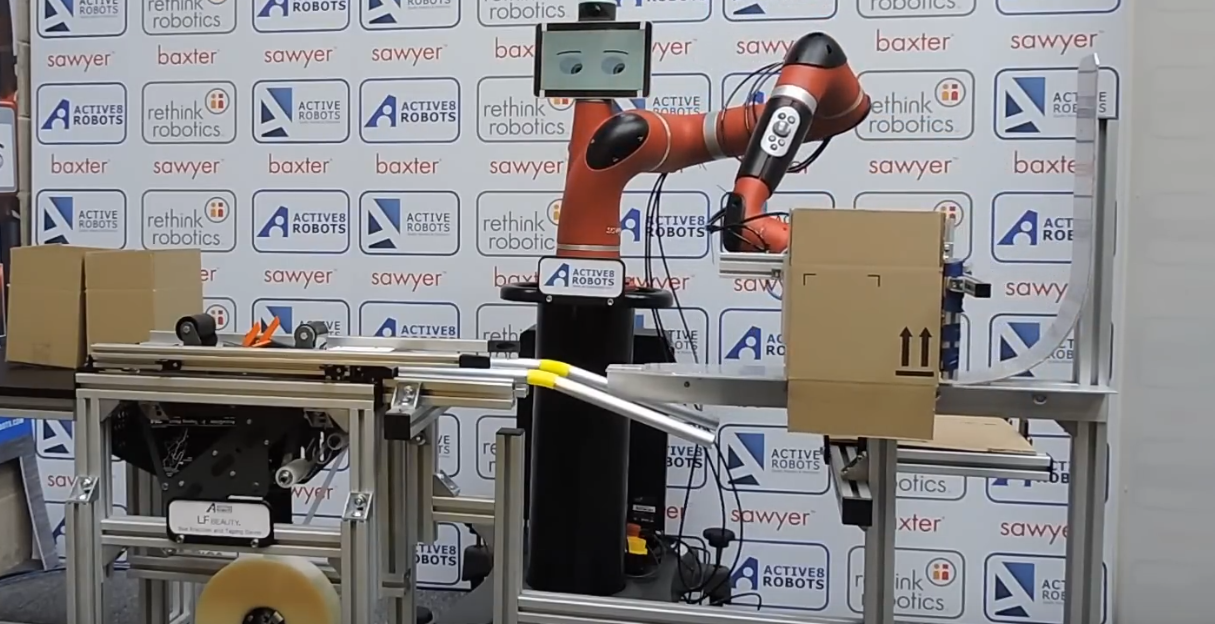
\includegraphics[width=\textwidth]{images/box.png}
  \end{columns}
\end{frame}

\section{期末專題提案}
\begin{frame}{機器手臂下棋}
  \Large 功能
  \normalsize \begin{itemize}
    \item 使用影像辨識技術辨識棋盤
    \item 透過Chess Engine計算下一步位置
    \item 機器手臂移動棋子
  \end{itemize}
\end{frame}




\begin{frame}[standout]
  Questions?
\end{frame}

\appendix


\begin{frame}[allowframebreaks]{參考文獻}

  \bibliography{demo}
  \bibliographystyle{abbrv}

  \begin{thebibliography}{9}
    \bibitem{ref1} \url{https://www.aboutamazon.com/news/operations/amazon-fulfillment-center-photo-tour}
    \bibitem{ref2} \url{https://www.youtube.com/watch?v=M3m5Oc8W9vk&t=1s}
    \bibitem{ref3} \url{https://www.youtube.com/watch?v=8nKPC-WmLjU&t=572s&pp=ygUZYW1hem9uIGZ1bGZpbGxtZW50IGNlbnRlcg\%3D\%3D}
  \end{thebibliography}

\end{frame}

\end{document}
